\chapter{Implementación}

Para la consecución de este proyecto, el desarrollo del software se ha dividido en una serie
de \textbf{hitos}. Un hito, en el desarrollo de software, simboliza un logro, un aspecto
del proyecto que se está cumpliendo conforme se planificó al comienzo del mismo, por tanto, 
éstos son los mejores indicadores del progreso del proyecto para alcanzar los objetivos
finales.\\

A cada hito se le asocia una serie de \textbf{issues} (problemas), los cuáles describen
aspectos a mejorar o solucionar del software durante su desarrollo. \\

Los hitos del proyecto son los siguientes:
\begin{enumerate}
    \item \textbf{\href{https://github.com/alexespana/TFG/milestone/1}{[M1]. Website
    creation}}: creación de la estructura principal de la aplicación web, con las
    principales páginas y funcionalidades. Esta parte será desarrollada en un entorno
    de desarrollo (servidor de desarrollo).
    \item \textbf{\href{https://github.com/alexespana/TFG/milestone/8}{[M2]. Database
    creation}}: creación de las principales tablas para modelar el problema, junto con
    los correspondientes formularios para la recogida de datos en la aplicación web.
    \item \textbf{\href{https://github.com/alexespana/TFG/milestone/2}{[M3]. Authentication}}
    : gestión de usuarios del sitio web, signup, signout, login, logout, cambiar
    contraseña e información de contacto para cada usuario así como third party (social)
    account authentication. 
    \item \textbf{\href{https://github.com/alexespana/TFG/milestone/3}{[M4]. Test behavior}}:
    realización de tests para comprobar el comportamiento de la aplicación.
    \item \textbf{\href{https://github.com/alexespana/TFG/milestone/4}{[M5]. Continuous
    integration}}: el software desarrollado debe integrarse con el posible software
    ya existente en el sitio web, asegurando el correcto funcionaminto de ambos.
    \item \textbf{\href{https://github.com/alexespana/TFG/milestone/5}{[M6]. Log system}}: 
    los eventos más importantes que ocurren en la aplicación deben ser grabados a través
    del uso de un servicio de log. Es conveniente capturar errores en un nivel superior
    de abstracción, evitando modificar código ya hecho.
    \item \textbf{\href{https://github.com/alexespana/TFG/milestone/6}{[M7]. API REST}}:
    el diseño y posterior implementación de la API REST que permita gestionar los recursos
    con los que trabaja la aplicación.
    \item \textbf{\href{https://github.com/alexespana/TFG/milestone/7}{[M8]. Deployment}}:
    el despliegue de la aplicación web en la nube debe realizarse utilizando un dominio
    público y un WSGI (Web Server Gateway Interface).
\end{enumerate}

Si desea tener una vista más general de los milestones, issues, commits, branches, etc del
proyecto puede visitar los siguientes enlaces:

\begin{itemize}
    \item \textbf{\href{https://github.com/alexespana/TFG/milestones}{Milestones}}
    \item \textbf{\href{https://github.com/alexespana/TFG/issues}{Issues}}
    \item \textbf{\href{https://github.com/alexespana/TFG/branches}{Branches}}
    \item \textbf{\href{https://github.com/alexespana/TFG/pulls}{Pull requests}}
\end{itemize}


\section{Website creation}
Para realizar la implementación de las distintas plantillas de la aplicación, se ha hecho
uso del sistema propio de plantillas de Django, llamado \textbf{Django template language},
que es muy parecido a JinJa2 y que está completamente implementado en los backends que
incluye de serie.\\

A la hora de pensar en un diseño para la aplicación web, se ha optado por un diseño
minimalista, que permita diferenciar fácilmente las distintas partes de la aplicación
junto con sus funcionalidades.\\

Es importante mencionar que todas las plantillas del proyecto hacen uso de una plantilla
base que contiene el navegador de la página y el pie de página, por lo que dicha plantilla base
sería tal que así:\\

    \begin{figure}[H]
        \centering
        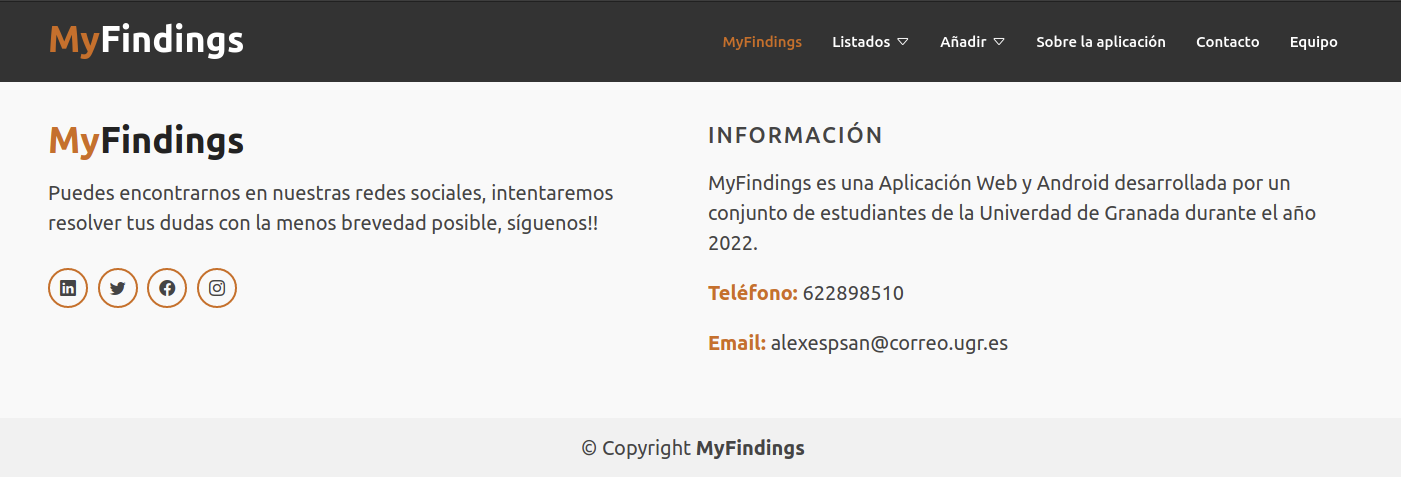
\includegraphics[scale=0.25]{imagenes/base.png}
        \caption{Plantilla base}
        \label{fig:base}
    \end{figure}

El resto de plantillas de este diseño son las que se describen en las secciones siguientes.

    \subsection{Home}
    Ésta es la página principal que se verá al entrar en la aplicación, prácticamente todo el
    diseño de ésta tiene relación con un componente de bootstrap llamado \textbf{Carousel}, que
    nos permite construir una especie de sliders en la vista con indicadores en la parte
    inferior. Además, cada uno de estos sliders puede tener texto asociado e imágenes de fondo,
    por lo que podemos ir cambiando el fondo completo de la página mediante el uso de javascript
    cada cierto tiempo predefinido. De esta forma, hacemos que entrar en la página sea una
    sensación agradable a primera vista. El \textbf{home} quedaría así:
    
        \begin{figure}[H]
            \centering
            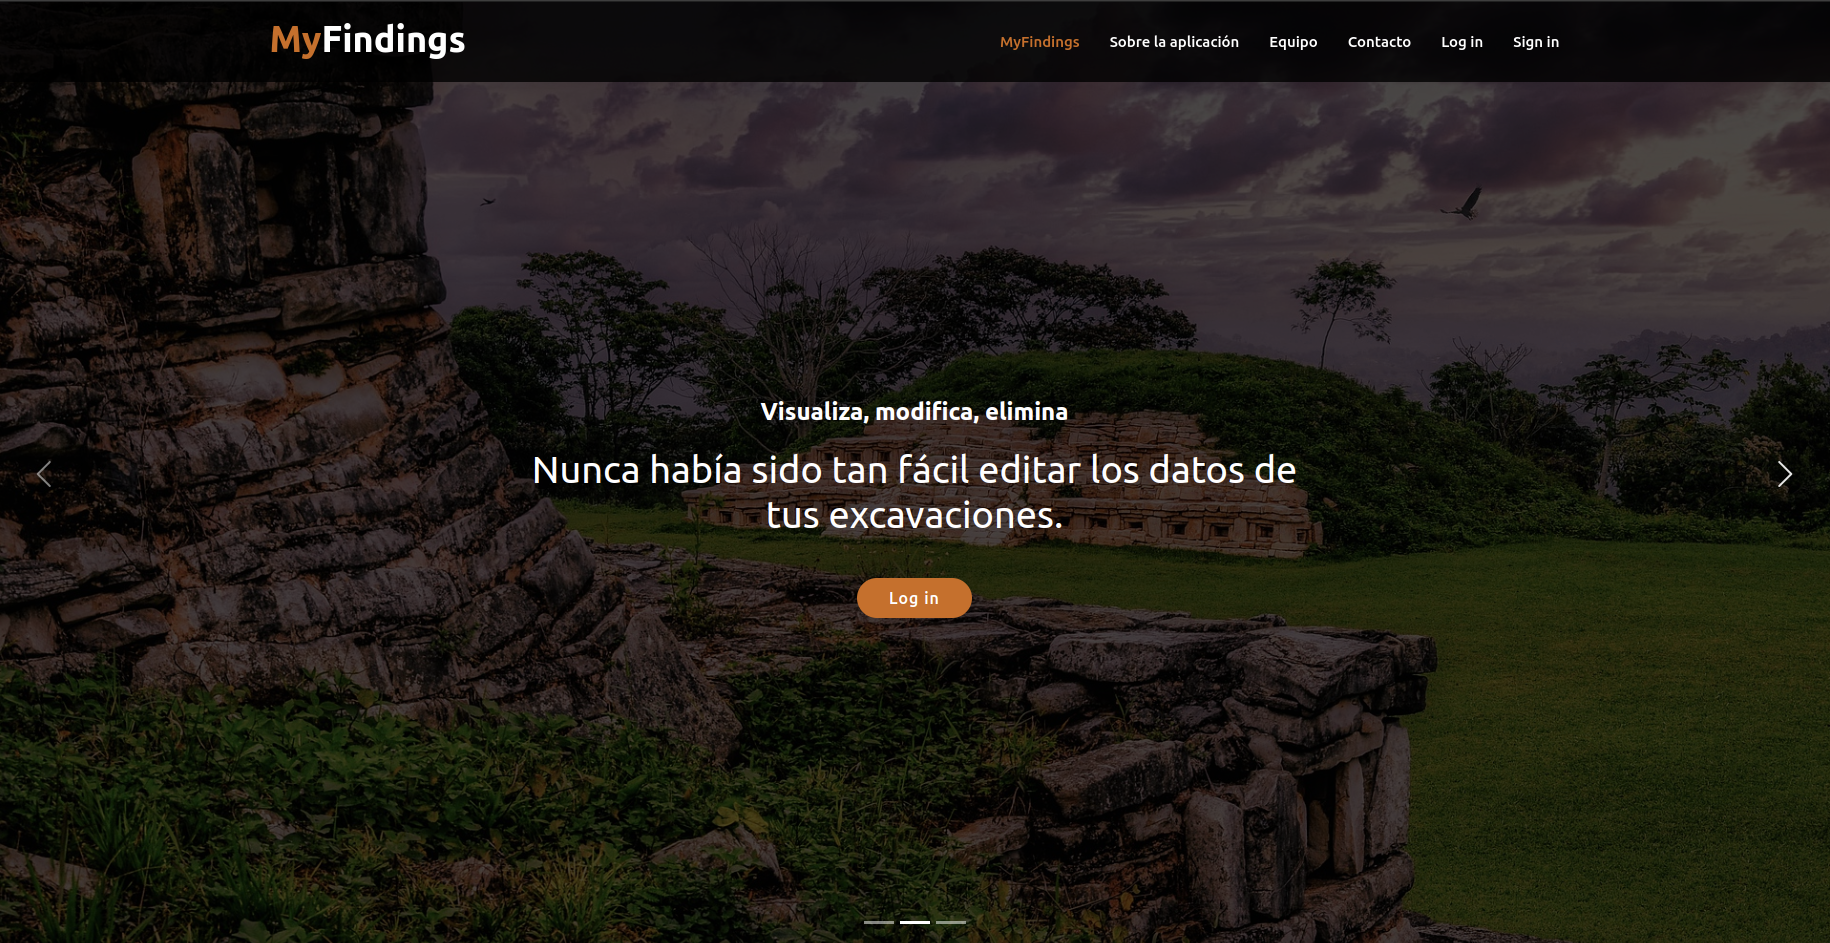
\includegraphics[scale=0.17]{imagenes/home.png}
            \caption{Home de la página}
            \label{fig:home}
        \end{figure}

    \subsection{Listados}
    Esta parte de la vista corresponderá a distintas vistas que servirán para listar en forma
    de \textbf{tablas} las distintas excavaciones, estancias, hechos, unidades estratigráficas
    (sedimentarias y construidas), fotografías, materiales (sedimentarios y construidos) e
    inclusiones.\\

    Principalmente corresponderá a tablas donde además de la información propia
    de los registros se muestren las posibilidades de editar y eliminar dichos registros
    residentes en la base de datos, que como dijimos en la sección de análisis, va a ser
    PostgreSQL. Esta parte de la implementación se explicará en secciones posteriores.

    \subsection{Añadir}
    Esta sección de la página web corresponderá a las distintas vistas (formularios) que
    servirán para añadir los distintos componentes relacionados con las excavaciones:
    excavaciones, estancias, hechos, unidades estratigráficas (sedimentarias y construidas),
    fotografías, materiales (sedimentarios y construidos) e inclusiones.\\

    Cada uno de estos formularios pedirá al usuario los datos completos de cada elemento del
    que se trate, por supuesto, con la posibilidad de dejar algún campo en blanco, aunque
    no sería lo más normal ya que en el servidor web la idea es rellenar de forma completa
    la información que se recopile en el registro de campo con la aplicación android, además
    de añadir otra información.

    \subsection{Sobre la aplicación}
    En esta página de la web se hace alusión brevemente a cuál es la principal motivación
    de crear este proyecto y cuales son las principales características que posee la
    aplicación: \textit{sincronización en tiempo real con la aplicación android, fácil
    adición, edición y eliminación de información de los distintos elementos, generación
    de informes a partir de la información de la base de datos, etc}.\\

    Dicha página quedaría de la siguiente forma:
        
        \begin{figure}[H]
            \centering
            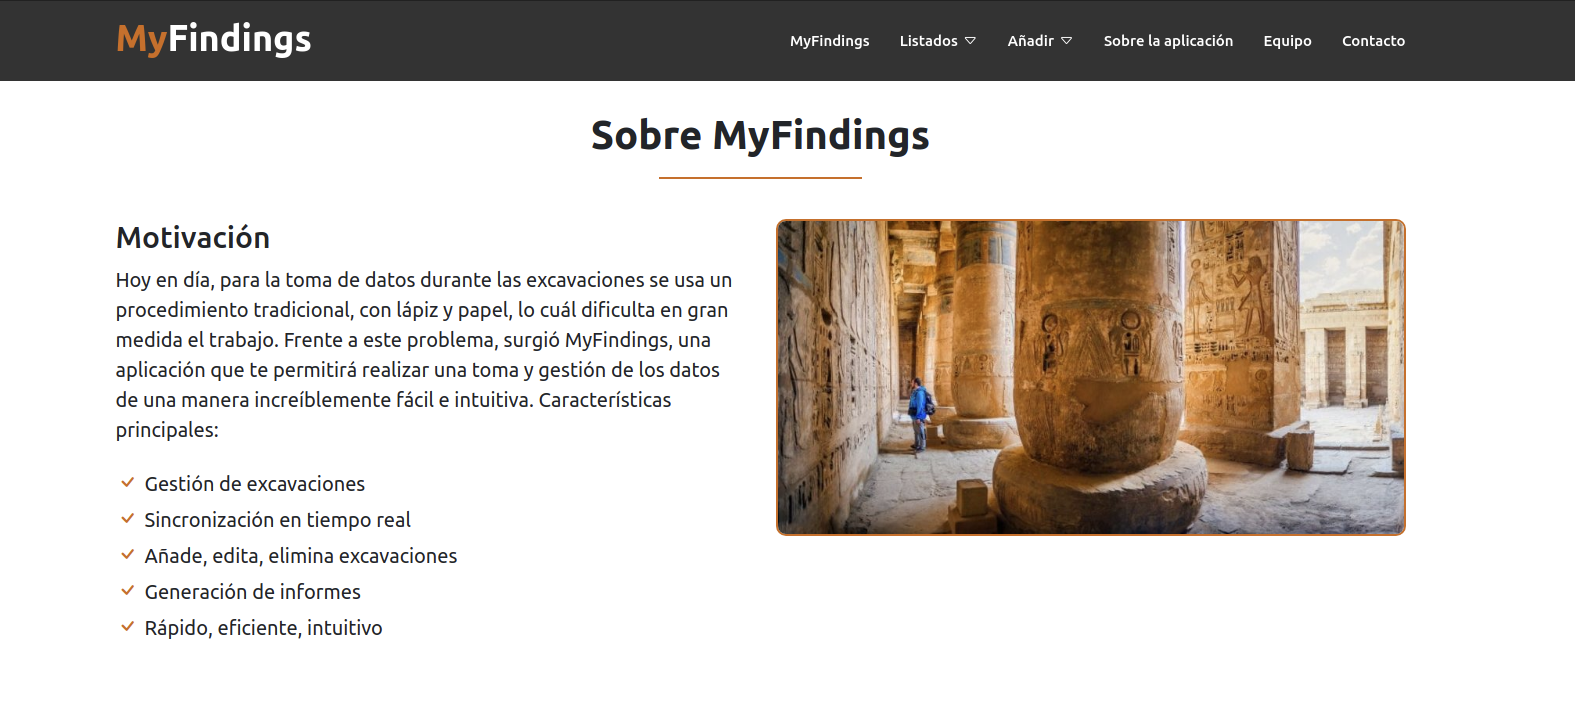
\includegraphics[scale=0.20]{imagenes/about.png}
            \caption{Sobre la aplicación}
            \label{fig:about}
        \end{figure}

    Como puede observarse, esta página está formada por dos rows, el primero, que se
    corresponde con el \textbf{headline} (común en muchas páginas) y el segundo, que está
    dividido en dos partes que usan 6 columnas de Bootstrap cada una, conteniendo la
    \textbf{motivación} y la \textbf{imagen}.

    \subsection{Equipo}
    Esta página contiene información sobre los componentes que hemos hecho posible este
    proyecto, en este caso, \textit{Joaquín García Venegas} y yo, \textit{Joaquín
    Alejandro España Sánchez}\\
    
    Por supuesto, ambos hacemos funciones totalmente distintas, por un lado la aplicación
    android y por otro la aplicación web, sobre lo que nos centraremos en este proyecto.
    Ambos componentes son diferentes, pero en su conjunto forman \textbf{MyFindings},
    un proyecto completamente funcional. La página quedaría tal que así:

        \begin{figure}[H]
            \centering
            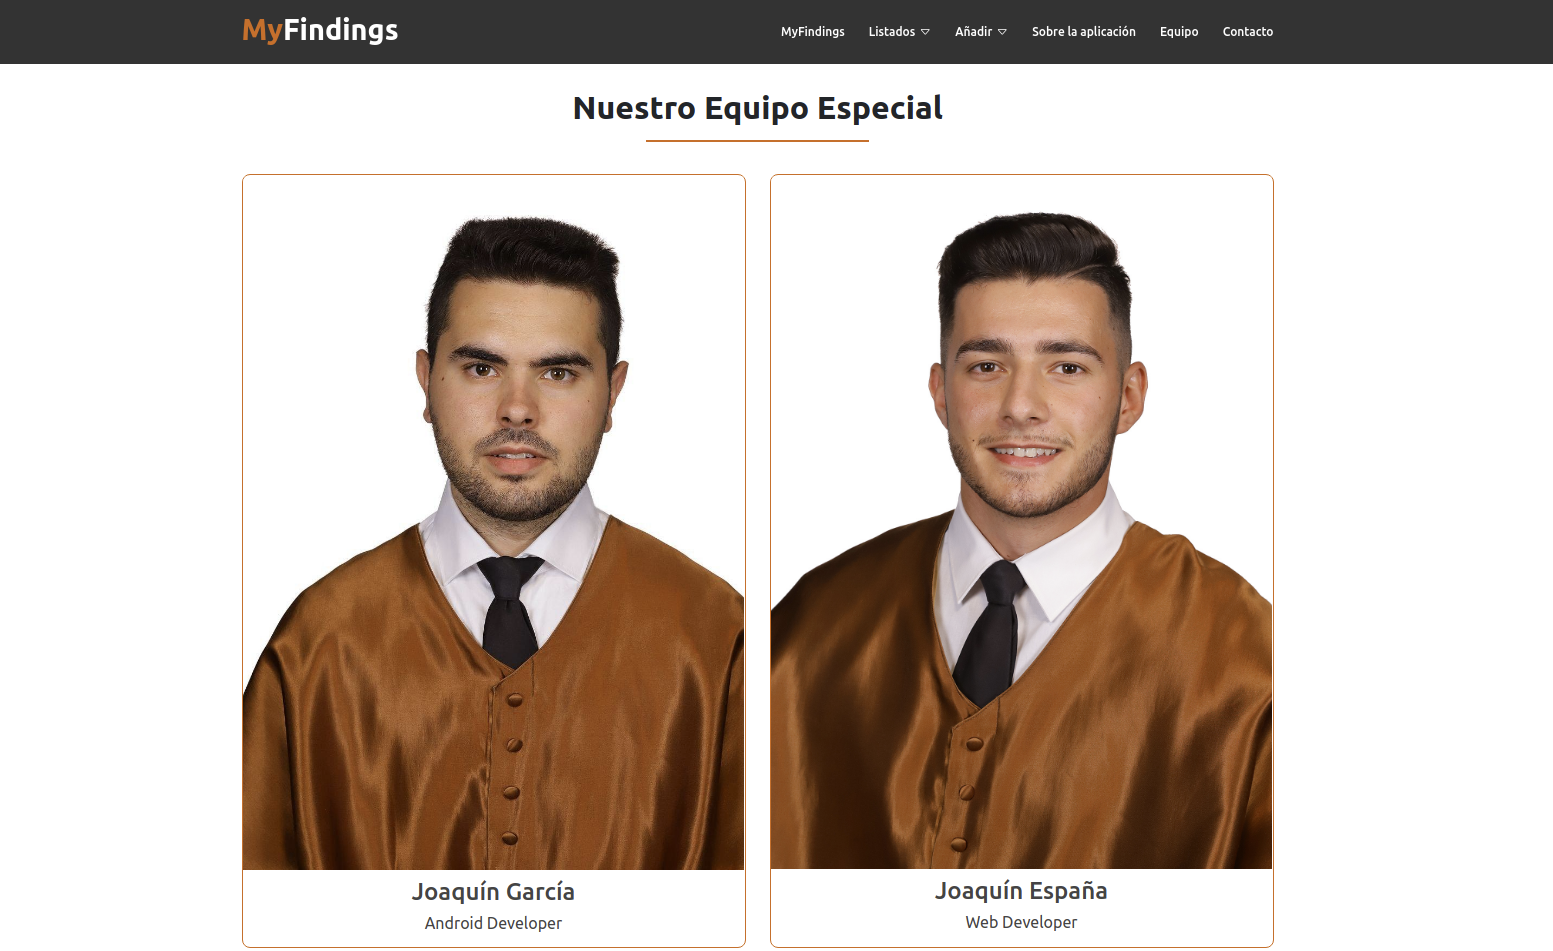
\includegraphics[scale=0.20]{imagenes/team.png}
            \caption{Equipo de MyFindings}
            \label{fig:team}
        \end{figure}

    En este caso se ha utilizado una estructura de página muy parecida a la anterior, utilizando
    dos rows, el primero para el \textbf{headline} y el segundo para los \textbf{miembros} del
    proyecto. Cabe mencionar el uso de la clase \textbf{border-box} en numerosas ocasiones en 
    el código, éste incorpora un border naranja al componente que lo posea.

    \subsection{Contacto}
    Finalmente, tenemos la página de contacto de la aplicación web, en ella podemos
    encontrar datos como el correo electrónico del desarrollador y su página de
    \href{https://github.com/alexespana/}{Github} o un mapa del lugar de residencia del
    programador, en este caso Granada.\\

        \begin{figure}[H]
            \centering
            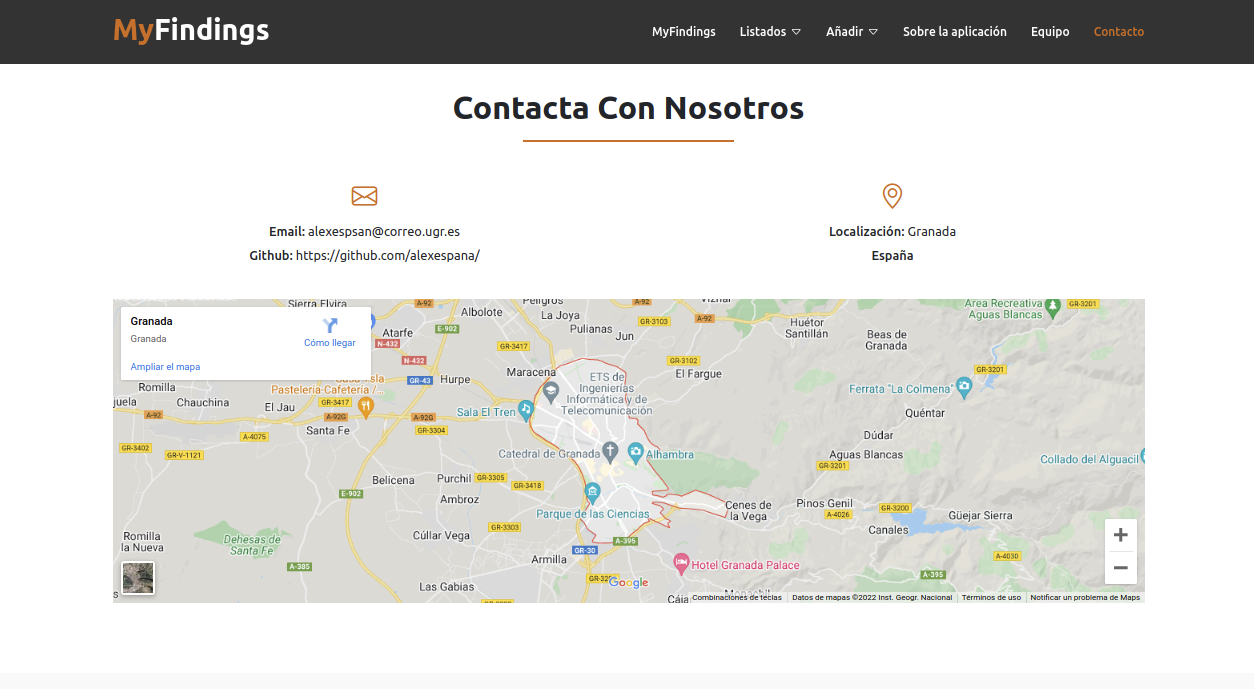
\includegraphics[scale=0.25]{imagenes/contact.png}
            \caption{Contacto de MyFindings}
            \label{fig:contact}
        \end{figure}

    Para realizar esta página se ha hecho uso de tres filas, la primera de ellas
    está destinada al \textbf{headline}, que como hemos visto, es común en otras páginas, 
    por lo que usan la misma clase de estilo CSS. La segunda a su vez está dividida en 
    dos partes utilizando cada una 6 columnas y finalmente la tercera fila ha sido
    destinada para el \textbf{iframe} de google maps cuyo código html ha sido extraído
    directamente de la aplicación web y puesto sobre el código.
